\documentclass[aspectratio=169]{beamer}
\usetheme{Singapore}
\addtobeamertemplate{navigation symbols}{}{%
    \usebeamerfont{footline}%
    \usebeamercolor[fg]{footline}%
    \hspace{1em}%
    \raisebox{1.4pt}[0pt][0pt]{\insertframenumber/\inserttotalframenumber}
}
\setbeamercolor{footline}{fg=blue!50}
\setbeamerfont{footline}{series=\bfseries}

\DeclareMathAlphabet{\digitsbb}{U}{bbold}{m}{n}

\usefonttheme[onlymath]{serif}

\usepackage{cmap}
\usepackage[english]{babel}
\usepackage[T1]{fontenc}
\usepackage[utf8]{inputenc}
\usepackage[kerning=true]{microtype}
\usepackage{lmodern}

\usepackage{amsmath}
\usepackage{amsfonts}
\usepackage{amssymb}
\usepackage{amsthm}

\usepackage{mathtools}
\usepackage{wrapfig}
\usepackage{enumitem}
\usepackage{tikz}
\usepackage{xcolor}
\usetikzlibrary{positioning}

\usepackage[
    backend=biber,
    style=numeric,
]{biblatex}
\usepackage{graphicx}
\usepackage[justification=centering]{caption}

\graphicspath{{../images/}}

\addbibresource{../report/report.bib}
\renewcommand*{\bibfont}{\footnotesize}

\AtBeginSection[]
{
  \begin{frame}
    \frametitle{Plan}
    \tableofcontents[currentsection]
  \end{frame}
}


\theoremstyle{definition}
\newtheorem*{exemple}{Example}



\title{\textbf{Extending Layerwise Relevance Propagation using Semiring Annotations}}

\author{%
  \texorpdfstring{%
    \begin{columns}
      \column{.5\linewidth}
      \centering
      \textbf{Antoine Groudiev} \\ L3, ENS Ulm
      \column{.5\linewidth}
      \centering
      \textbf{Silviu Maniu} -- Supervisor \\ SLIDE Team, LIG
    \end{columns}
 }
 {Antoine Groudiev, Silviu Maniu}
}

\date{\today}

\begin{document}
\frame{\titlepage}

%\begin{frame}{Plan}
%    \tableofcontents
%\end{frame}

\section{Introduction}
\subsection{Problem statement}
\begin{frame}{Problem statement}
    \begin{figure}
        \centering
        \begin{tikzpicture}
            \node at (0, 0) {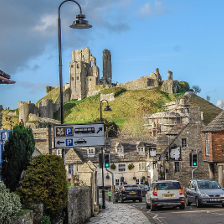
\includegraphics[width=.4\textwidth]{castle.jpg}};
            \node at (6.5, 0) {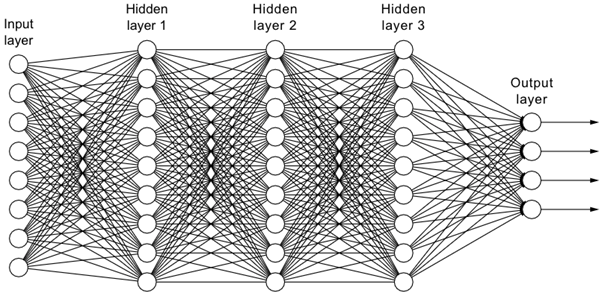
\includegraphics[width=.5\textwidth]{mlp.png}};

            \node at (11, -.3) {"\texttt{castle}"};
        \end{tikzpicture}
    \end{figure}
\end{frame}

\subsection{Layerwise Relevance Propagation}
\begin{frame}{Layerwise Relevance Propagation \cite{montavon-lrp}}
    \begin{figure}[H]
        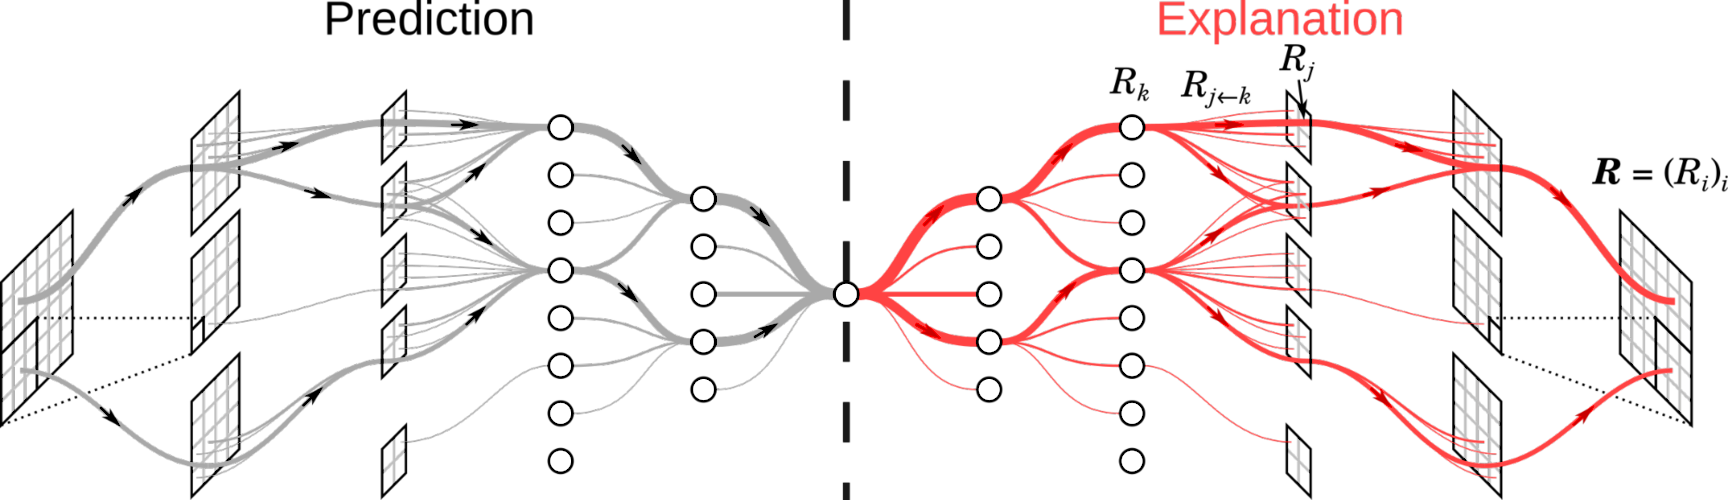
\includegraphics[width=\textwidth]{LRP.png}
    \end{figure}
\end{frame}

\begin{frame}{Layerwise Relevance Propagation}{Initialization}
    Initialization:
    \begin{equation}
        R^{(L)}_i = \begin{cases*}
            \textcolor{red}{a^{(L)}_i} & if $i = y$ (the class we want)\\
            0 & otherwise
        \end{cases*}
    \end{equation}

    \begin{figure}
        \centering
        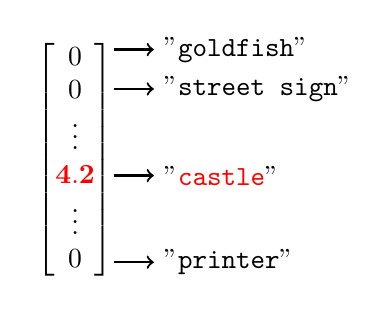
\begin{tikzpicture}
            \node at (0, 0) {$
                \begin{bmatrix}
                    0\\
                    0\\
                    \vdots\\
                    \textcolor{red}{\bf 4.2}\\
                    \vdots\\
                    0
                \end{bmatrix}
            $};
            \draw [->, thick] (0.5, 1.4) -- ++ (.5, 0) node[right] {"\texttt{goldfish}"};
            \draw [->, thick] (0.5, .9) -- ++ (.5, 0) node[right] {"\texttt{street sign}"};
            \draw [->, thick] (0.5, -.2) -- ++ (.5, 0) node[right] {"\texttt{\textcolor{red}{castle}}"};
            \draw [->, thick] (0.5, -1.3) -- ++ (.5, 0) node[right] {"\texttt{printer}"};
        \end{tikzpicture}
    \end{figure}
\end{frame}

\begin{frame}{Layerwise Relevance Propagation}{Propagation}
    LRP-0 rule:
    \begin{equation}
        R^{(l)}_j = \sum_{k}\frac{a^{(l)}_jw_{j, k}}{\sum_{j'}a^{(l)}_{j'}w_{j', k}} \cdot R^{(l+1)}_k
    \end{equation}
    \begin{figure}
        \centering
        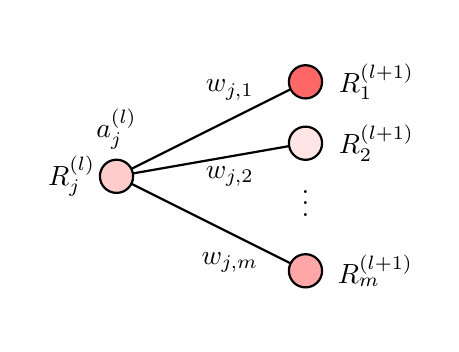
\begin{tikzpicture}[scale=.6]
            \draw[thick] (0,0) -- (4, 2) node[above=.12, pos=.6] {$w_{j,1}$};
            \draw[thick] (0,0) -- (4, .7) node[below, pos=.6] {$w_{j,2}$};
            \draw[thick] (0,0) -- (4, -2) node[below=.12, pos=.6] {$w_{j,m}$};

            \node at (0, 1) {$a_j^{(l)}$};
            \draw[thick, fill=red!20,circle,minimum size=15] (0, 0) circle (10pt) node[left] {$R_j^{(l)}$};

            \draw[thick, fill=red!60,circle,minimum size=15] (4, 2) circle (10pt) node[right=.2] {$R_1^{(l+1)}$};
            \draw[thick, fill=red!10,circle,minimum size=15] (4, .7) circle (10pt) node[right=.2] {$R_2^{(l+1)}$};
            \node at (4, -.4) {$\vdots$};
            \draw[thick, fill=red!35,circle,minimum size=15] (4, -2) circle (10pt) node[right=.2] {$R_m^{(l+1)}$};
        \end{tikzpicture}
    \end{figure}
    Other rules exist (LRP-$\varepsilon$, LRP-$\gamma$, $z^\mathcal{B}$)
\end{frame}

\begin{frame}{LRP Results visualization}{Multilayer Perceptron on MNIST dataset}
    \begin{figure}[ht]
        \centering
        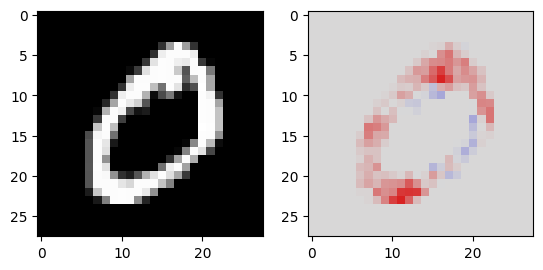
\includegraphics[width=.6\textwidth]{mnist-lrp.png}
        \caption{Reference image and relevance for the class 0}
    \end{figure}
\end{frame}

\begin{frame}{LRP Results visualization}{VGG-16 on ImageNet dataset}
    \begin{figure}[ht]
        \begin{minipage}[c]{0.45\linewidth}
            \centering
            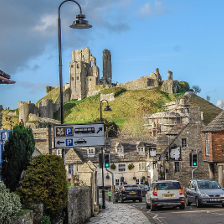
\includegraphics[width=.8\textwidth]{castle.jpg}
            \caption{Reference image}
        \end{minipage}
        \hspace{0.25cm}
        \begin{minipage}[c]{0.45\linewidth}
            \centering
            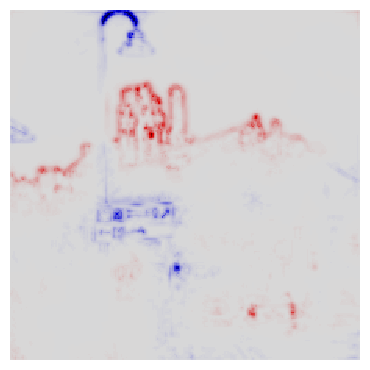
\includegraphics[width=.8\textwidth]{castle-lrp.png}
            \caption{Relevance for the class "\texttt{castle}"}
        \end{minipage}
    \end{figure}
\end{frame}

% \begin{frame}{Pertinence of LRP results}
%     \begin{figure}
%         \centering
%         \begin{tikzpicture}
%             \draw[->, thick] (-6.5, 1) -- ++ (3, 0) node [above, pos=.5] {\small Image label (0)};
%             \draw[->, thick] (-6.5, -1.5) -- ++ (3, 0) node [below, pos=.5] {\small Useless digit};
%             \node at (0, 0) {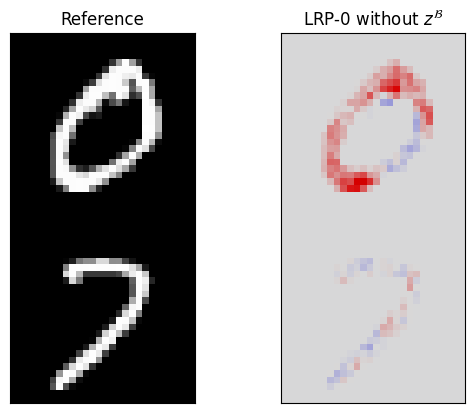
\includegraphics[width=.5\textwidth]{dmnist-lrp.png}};
%         \end{tikzpicture}
%     \end{figure}
% \end{frame}

\subsection{Semiring-based provenance annotations}
\begin{frame}{Semiring-based provenance annotations \cite{green-2007,ramusat-prov}}
    \begin{definition}[Semiring]
        A semiring $(\mathbb{K}, \oplus, \otimes, \digitsbb{0}, \digitsbb{1})$ is such that:
        \begin{itemize}[label=--, noitemsep]
            \item $\otimes$ distributes over $\oplus$,
            \item $(\mathbb{K}, \oplus, \digitsbb{0})$ is a commutative monoid,
            \item $(\mathbb{K}, \otimes, \digitsbb{1})$ is a monoid such that $\digitsbb{0}$ is absorbing
        \end{itemize}
    \end{definition}

    \begin{exemple}
        The following structures are semirings:
        \begin{itemize}[label=--, noitemsep]
            \item Real semiring: $(\mathbb{R}, +, \times, 0, 1)$
            \item Boolean semiring: $(\{\bot, \top\}, \lor, \land, \bot, \top)$
            \item Counting semiring: $(\mathbb{N}, +, \times, 0, 1)$
            \item Viterbi semiring: $([0, 1], \max, \times, 0, 1)$
        \end{itemize}
    \end{exemple}
\end{frame}

\section{Extending LRP}
% \begin{frame}{Simplifying LRP rule}
%     Remove the denominator:
%     \begin{equation*}
%         R^{(l)}_j = \sum_k\frac{a^{(l)}_jw_{j, k}^{(l)}}{\sum_{j'}a^{(l)}_{j'}w_{j', k}^{(l)}} R^{(l+1)}_k \quad \longrightarrow \quad R^{(l)}_j = \sum_{k} a^{(l)}_jw_{j, k}^{(l)} \cdot R^{(l+1)}_k
%     \end{equation*}
%     \newline{}
%     Use only LRP-0 rule (no $\varepsilon$, $\gamma$, $z^\mathcal{B}$, \dots)
% \end{frame}

\subsection{Rules modification}
\begin{frame}{Semiring generalization of the LRP rule}
    Consider a semiring $(\mathbb{K}, \oplus, \otimes, \digitsbb{0}, \digitsbb{1})$

    Conversion function:
    \begin{equation*}
        \Theta : \mathbb{R} \longrightarrow \mathbb{K}
    \end{equation*}
    Initialization:
    \begin{equation}
        R^{(L)}_i = \begin{cases*}
            \digitsbb{1} & if $i = y$\\
            \digitsbb{0} & otherwise
        \end{cases*}
    \end{equation}
    Propagation rule:
    \begin{equation}
        R^{(l)}_j = \bigoplus_k \Theta\left(
            \frac{a^{(l)}_jw_{j, k}}{\sum_{j'}a^{(l)}_{j'}w_{j', k}} 
        \right) \otimes R^{(l+1)}_k
    \end{equation}
\end{frame}

\subsection{MNIST dataset}
\begin{frame}{Boolean Semiring}{\large $(\{\bot, \top\}, \lor, \land, \bot, \top)$}
    \begin{equation*}
        \Theta = x \longmapsto \begin{cases*}
            \top & if $x\geq\theta$\\
            \bot & otherwise
        \end{cases*}
    \end{equation*}

    \begin{figure}[H]
        \centering
        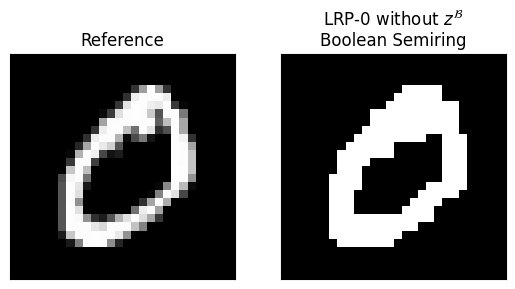
\includegraphics[width=.5\textwidth]{boolean.png}
    \end{figure}
\end{frame}

% \begin{frame}{Influence of the thresholds}
%     \begin{figure}
%         \centering
%         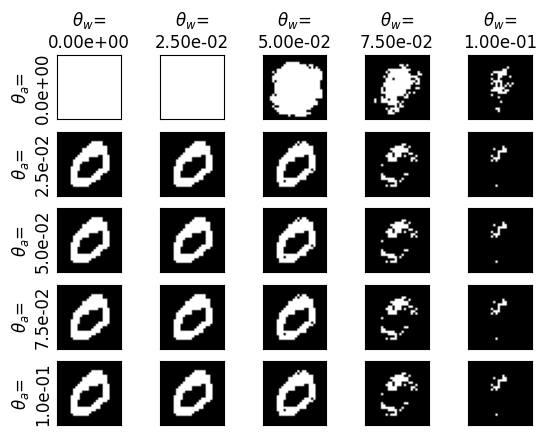
\includegraphics[width=.6\textwidth]{boolean-threshold.png}
%     \end{figure}
% \end{frame}

\begin{frame}{Counting Semiring}{\large $(\mathbb{N}, +, \times, 0, 1)$}
    \begin{equation*}
        \Theta = x \longmapsto \begin{cases*}
            1 & if $x\geq\theta$\\
            0 & otherwise
        \end{cases*}
    \end{equation*}

    \begin{figure}[H]
        \centering
        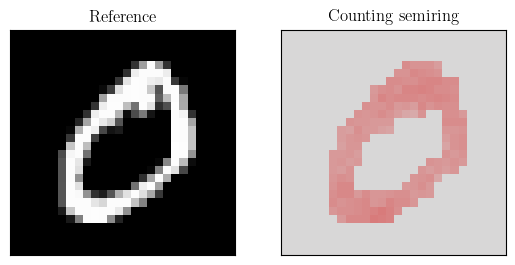
\includegraphics[width=.5\textwidth]{counting.png}
    \end{figure}
\end{frame}

\begin{frame}{Viterbi Semiring}{\large $([0, 1], \max, \times, 0, 1)$}
    \begin{equation*}
        R^{(l)}_j = \max_k \underbrace{\left(\frac{\left|a^{(l)}_jw_{j, k}^{(l)}\right|}{\max_{j'} \left|a^{(l)}_{j'}w_{j', k}^{(l)}\right|}\right)}_{\in[0, 1]} \cdot R^{(l+1)}_k
    \end{equation*}

    \begin{figure}[H]
        \centering
        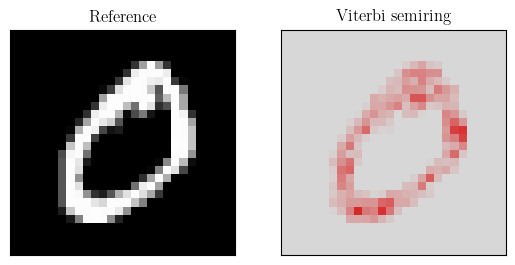
\includegraphics[width=.5\textwidth]{viterbi.png}
    \end{figure}
\end{frame}

\subsection{VGG-16 network}
\begin{frame}{Boolean semiring}
    \begin{figure}[H]
        \centering
        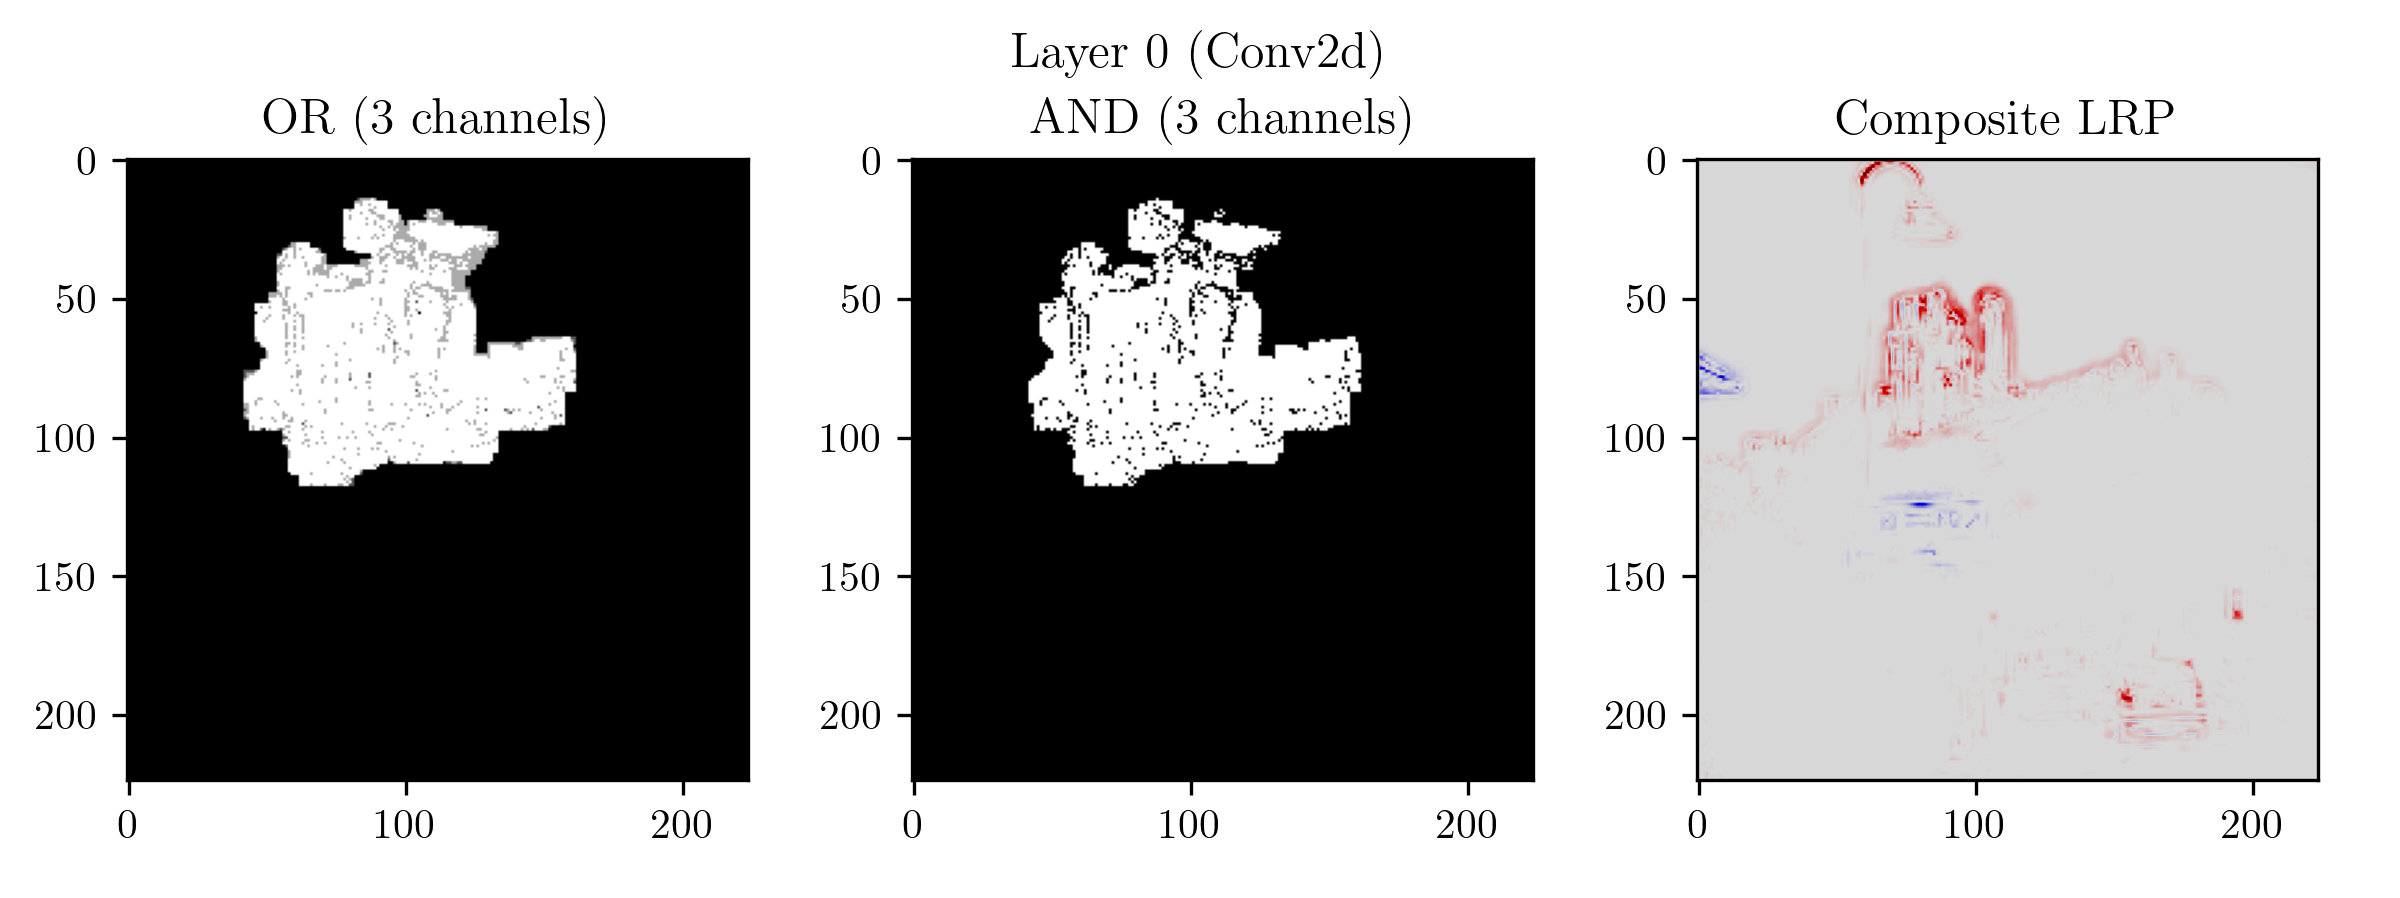
\includegraphics[width=\textwidth]{vgg-boolean.png}
    \end{figure}
\end{frame}

\begin{frame}{Counting semiring}
    \begin{figure}[H]
        \centering
        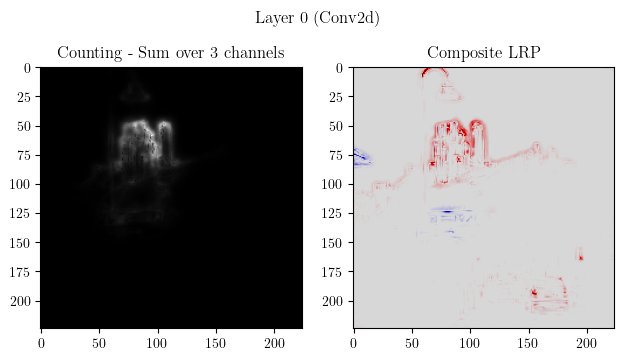
\includegraphics[width=.8\textwidth]{vgg-counting.png}
    \end{figure}
\end{frame}

\section{Applications}
\subsection{Image mask computation}
\begin{frame}{Class-wise mask -- Boolean semiring}
    \begin{figure}
        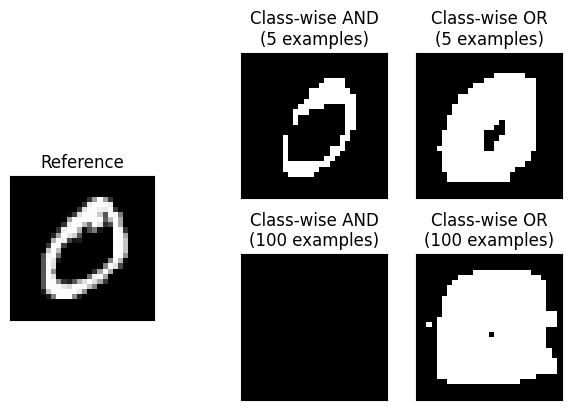
\includegraphics[width=.65\textwidth]{boolean-mask.png}
    \end{figure}
\end{frame}

\begin{frame}{All classes mask -- Boolean semiring}
    \begin{figure}
        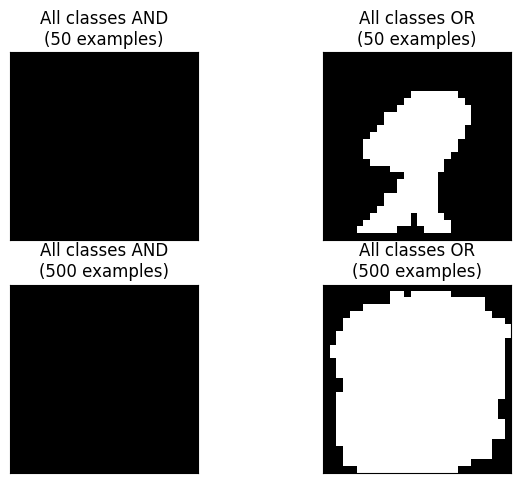
\includegraphics[width=.5\textwidth]{boolean-mask-all.png}
    \end{figure}
\end{frame}

\begin{frame}{Class-wise mask -- Counting semiring}
    \begin{figure}
        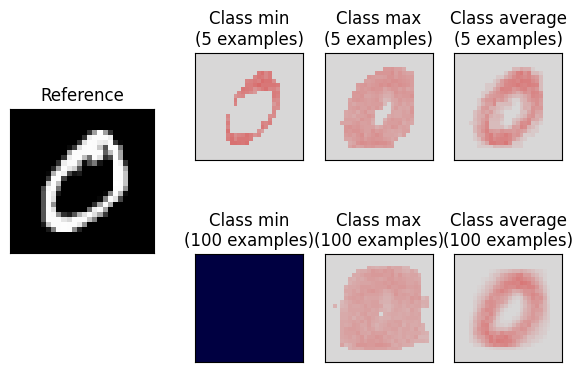
\includegraphics[width=.75\textwidth]{counting-mask.png}
    \end{figure}
\end{frame}

\begin{frame}{All classes mask -- Counting semiring}
    \begin{figure}
        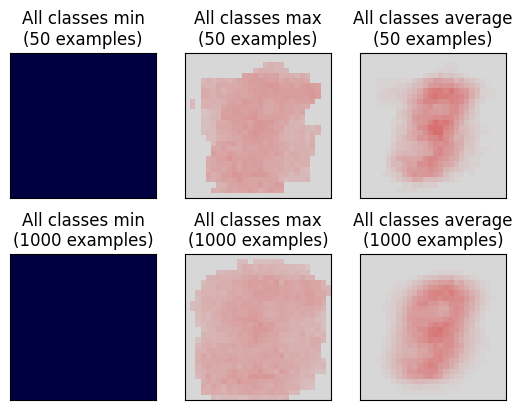
\includegraphics[width=.6\textwidth]{counting-mask-all.png}
    \end{figure}
\end{frame}

\begin{frame}{Comparison to dataset mean}
    \begin{figure}
        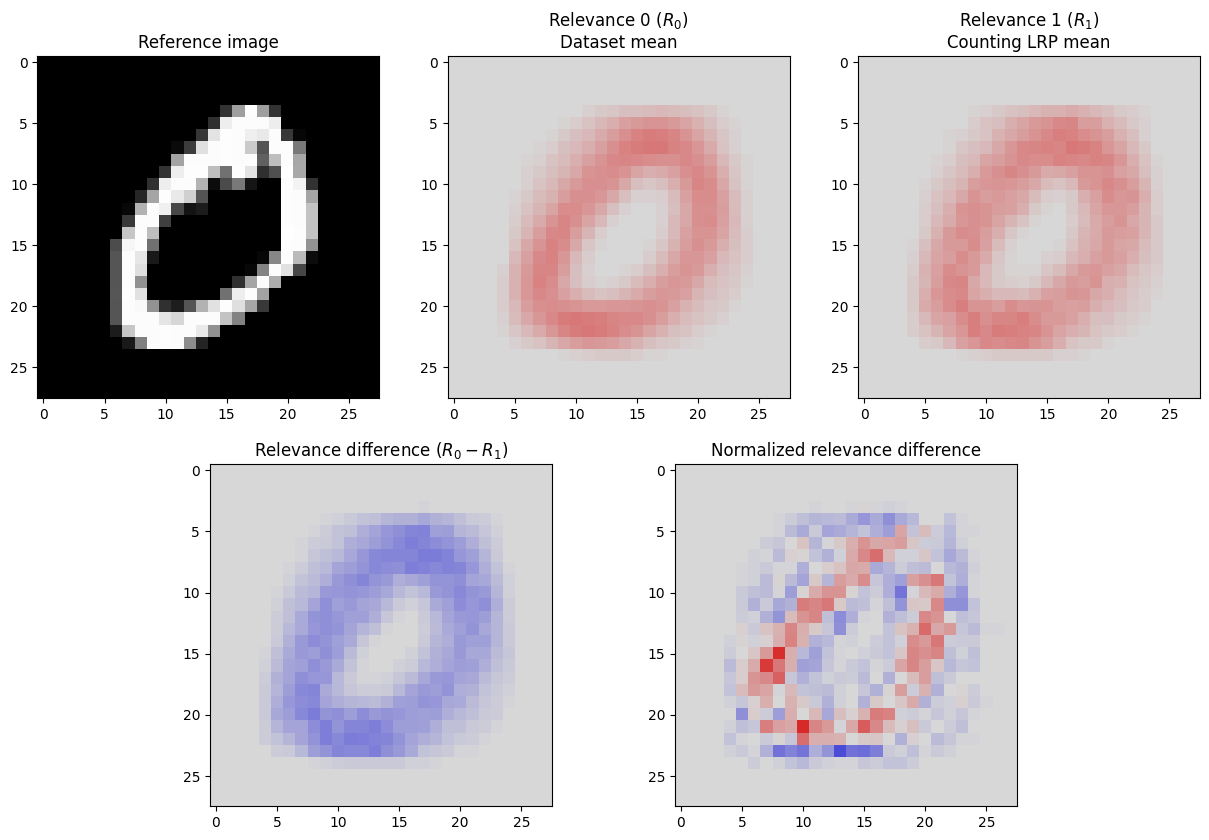
\includegraphics[width=.7\textwidth]{dataset-relevance-cmp.png}
    \end{figure}
\end{frame}

\subsection{Network pruning using LRP ranking}
\begin{frame}{Network pruning using LRP ranking}
    \begin{figure}[ht]
        \begin{minipage}[c]{0.55\linewidth}
            \centering
            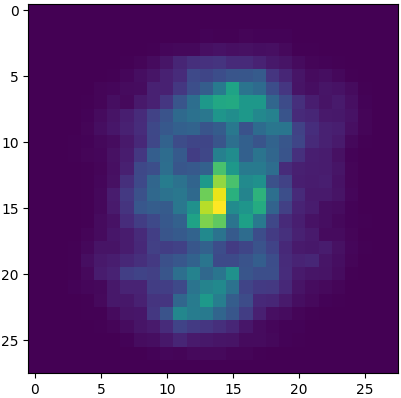
\includegraphics[width=.6\textwidth]{relevance-mean.png}
            \caption{Relevance mean over the training dataset (Input layer)}
        \end{minipage}
        \hspace{0.5cm}
        \begin{minipage}[c]{0.35\linewidth}
            \centering
            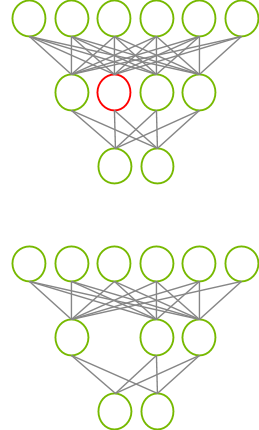
\includegraphics[width=.7\textwidth]{pruning.png}
        \end{minipage}
    \end{figure}
\end{frame}

\begin{frame}
    \begin{figure}
        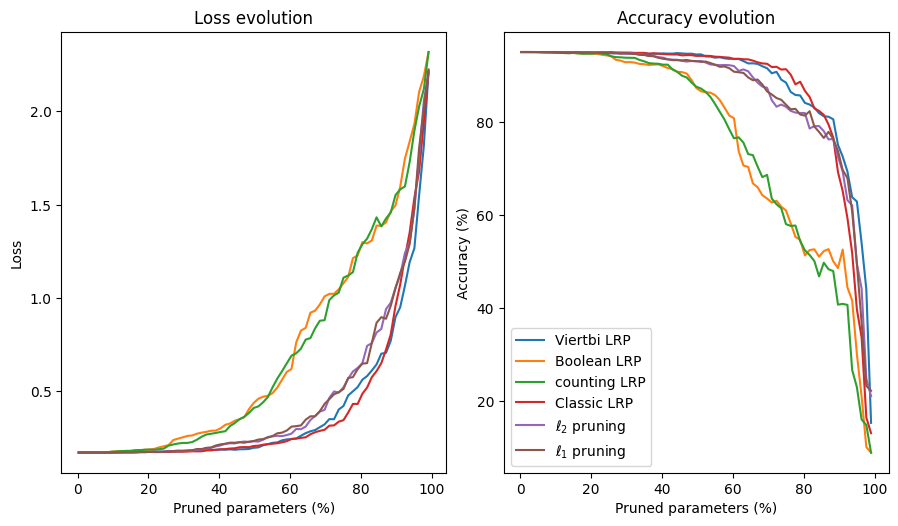
\includegraphics[width=.9\textwidth]{pruning-graph-large.png}
    \end{figure}
\end{frame}

\subsection{Comparison to image perturbation}
\begin{frame}{Comparison to image perturbation \cite{fong2017interpretable}}
    \begin{figure}
        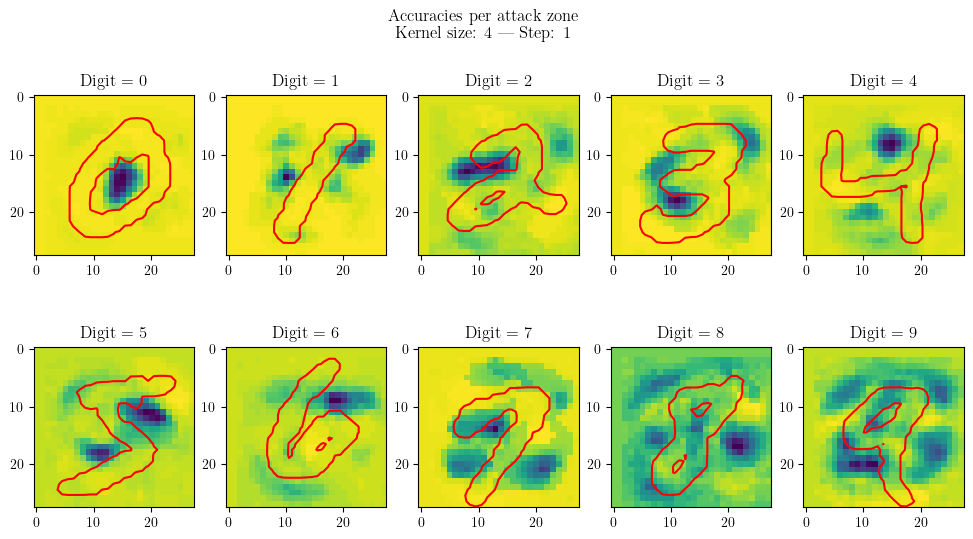
\includegraphics[width=.75\textwidth]{attacks.png}
        \caption{Accuracies per attack zone}
    \end{figure}
\end{frame}

\begin{frame}
    \begin{figure}[H]
        \hspace*{-.5cm}
        \begin{minipage}{.49\textwidth}
            \centering
            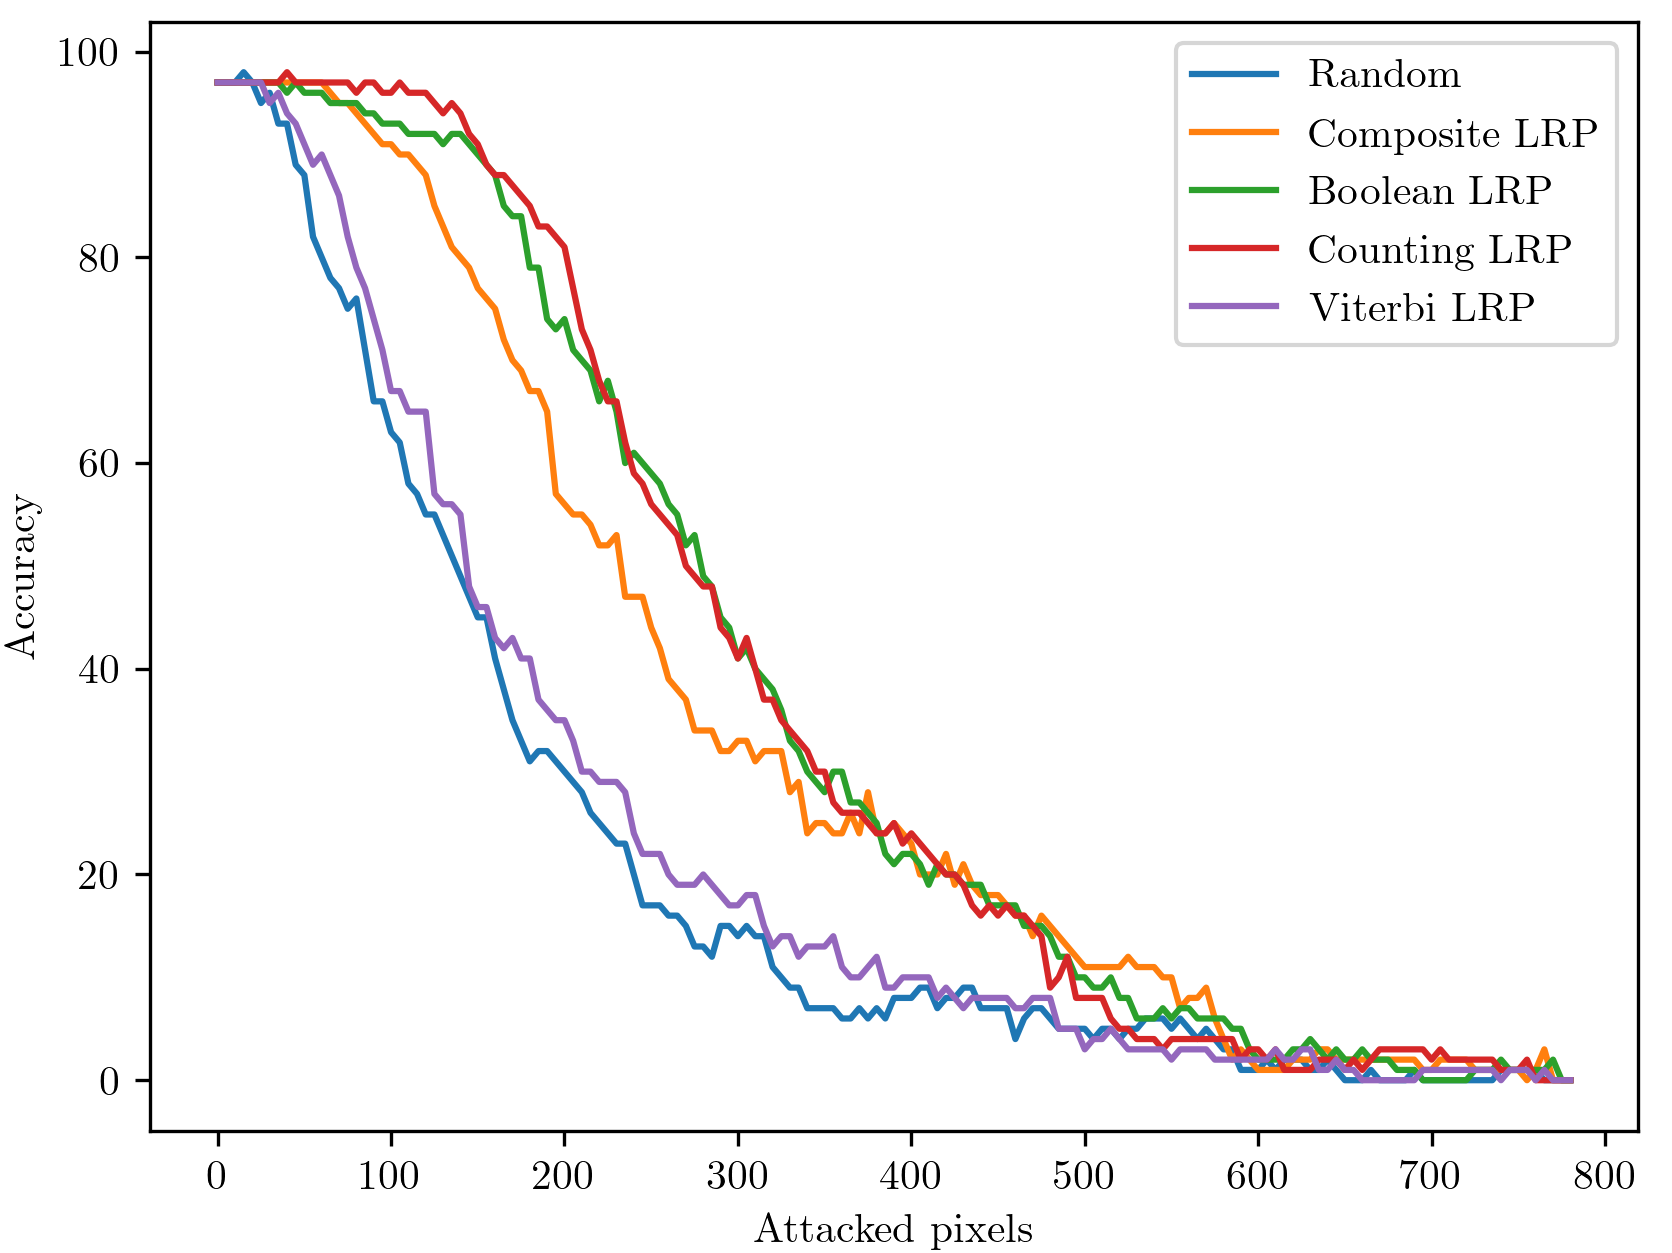
\includegraphics[width=1.1\textwidth]{attack-graph-1.png}
        \end{minipage}
        \begin{minipage}{.49\textwidth}
            \centering
            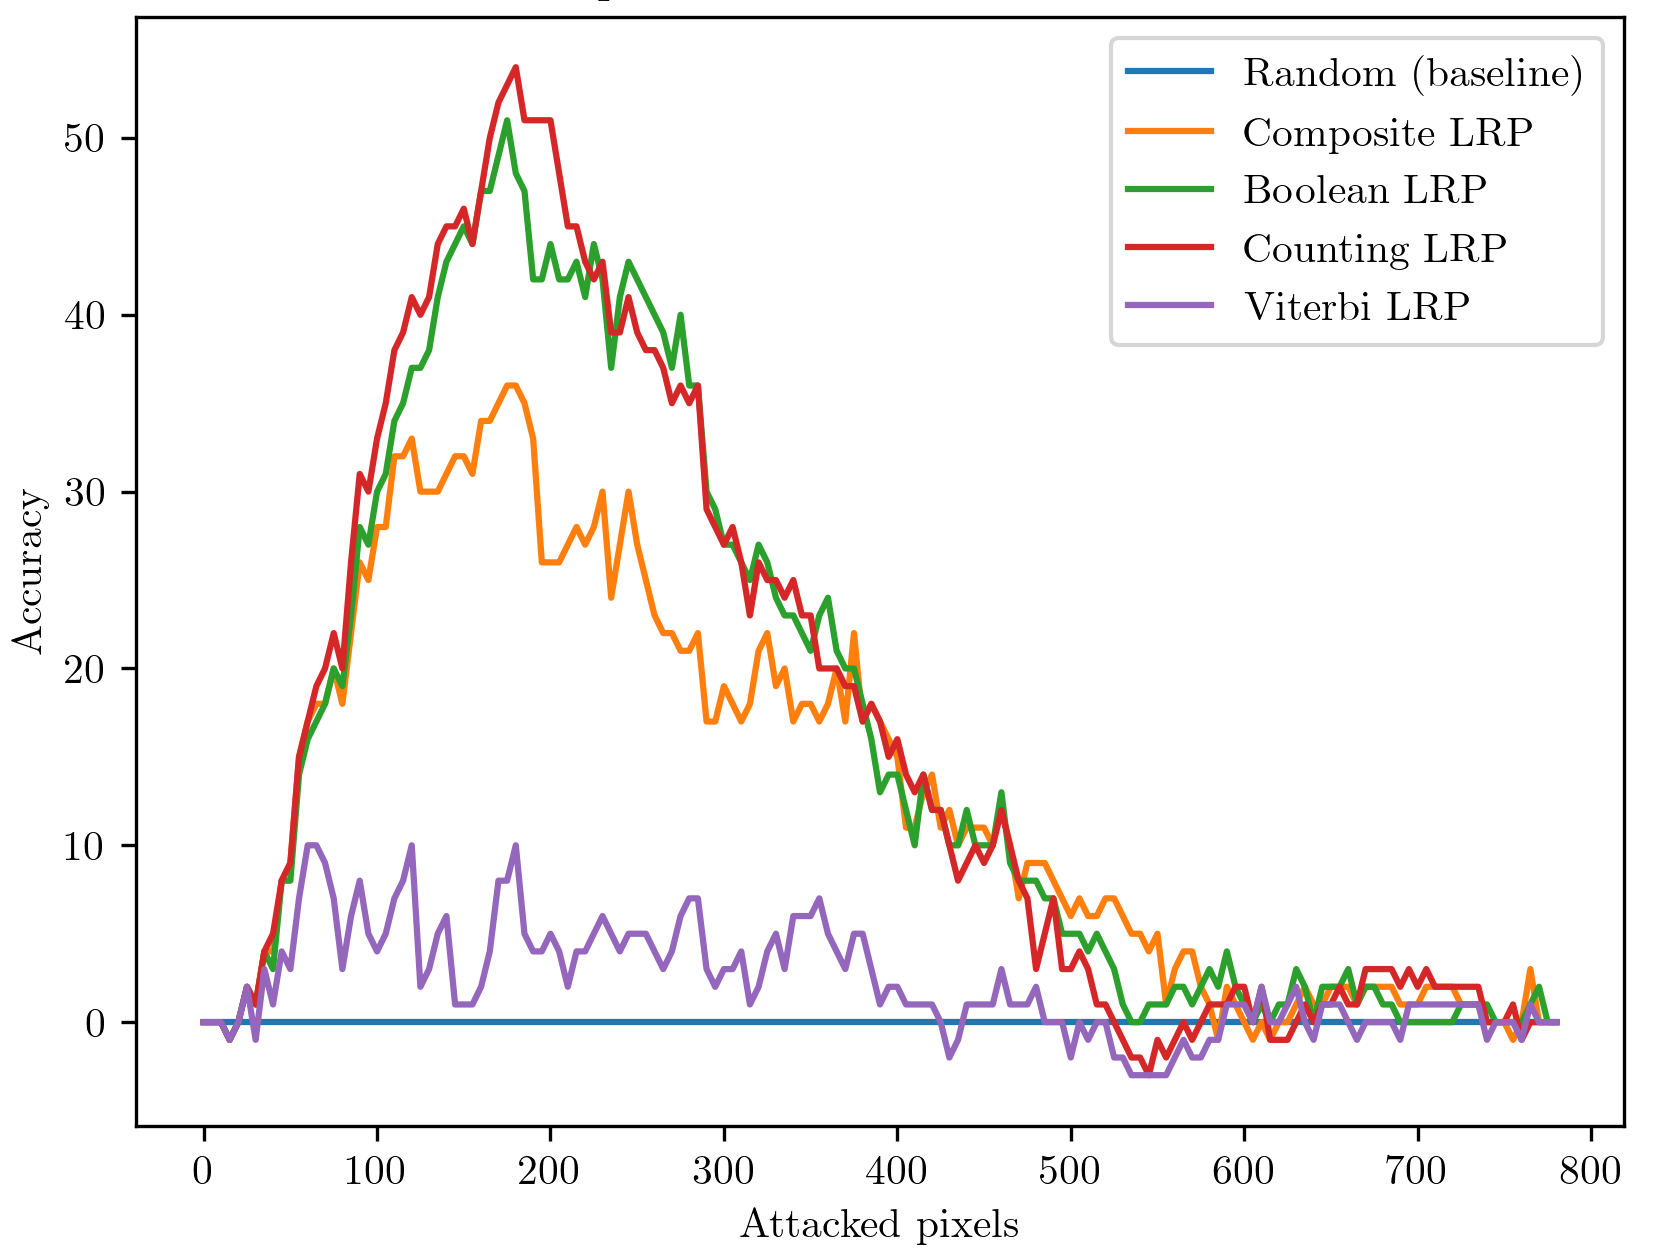
\includegraphics[width=1.1\textwidth]{attack-graph-2.png}
        \end{minipage}
        \caption{Accuracy drop for multiple pixels attacks strategies.}
        \label{fig:attack-graphs}
    \end{figure}
\end{frame}

\begin{frame}[allowframebreaks]
    \nocite{*}
    \printbibliography
\end{frame}

\end{document}